\documentclass[11pt, a4paper]{article}

\usepackage[english]{babel}
\usepackage[utf8]{inputenc}
\usepackage{amsmath}
\usepackage{graphicx}
\usepackage[colorinlistoftodos]{todonotes}
\usepackage{fancyhdr}
\usepackage{geometry}
\usepackage{caption}
\usepackage{apacite}
\usepackage[toc,page]{appendix}
\usepackage{etoolbox}
\usepackage{svg}

 \geometry{
 a4paper,
 total={170mm,257mm},
 left=25.4mm,
 right=25.4mm,
 top=25.4mm,
 bottom=25.4mm
 }

 \setlength\parindent{0pt}

\pagestyle{fancy}
\fancyhead{}
\lhead{Anders Havbro Hjulmand (201910185)}
\fancyfoot{}
\lfoot{Bachelor Thesis in Cognitive Science}
\rfoot{Page \thepage}

\newcommand{\figureshrinker}{\vspace{-3cm}}

\title{Mapping Individual Semantic Spaces using the Demonstrative Choice Task} \\ \\

\author{Anders Havbro Hjulmand (201910585)\\ \\ \\
Supervisor: Mikkel Wallentin\\ \\ 
Bachelor Thesis in Cognitive Science\\ \\
School of Communication and Culture, University of Aarhus}

\date{\today}

\begin{document}
\maketitle

\begin{abstract}
Demonstrative choice (e.g. \textit{this} or \textit{that}) is influenced by a range of factors that emerges from the relationship between the speaker and the referent. These include physical distance, ownership, familiarity, valence, and the self. While previous studies have focused on factors that are common among participants, individual differences in demonstrative use remain yet to be systematically investigated. This study used the Demonstrative Choice Task (DCT) to map the position of 480 words in the semantic space of 3,014 participants. After pairing words with demonstratives, participants completed short questionnaires for depression, anxiety, and Big Five personality traits. It was found that the DCT successfully mapped individual differences in semantic landscapes. Depressed and anxious individuals used more proximal demonstratives (\textit{this}) for words that evoked fear, sadness, and disgust, and they used more distal demonstratives (\textit{that}) for positive words. Furthermore, participants’ response patterns in the DCT were found to predict depression and anxiety. Many statistical models generalized to novel data, indicating that similar results are likely to be replicated in subsequent studies. The findings suggest that demonstrative choice is influenced by the way experiences, memories, personality traits, mental health, etc. shape the individual semantic landscape. Demonstratives can therefore reveal core aspects of individual semantic knowledge, underpinning their role as a powerful interface between language, cognition, and mental illnesses. Carefully selecting the set of words in future studies may increase the predictive power of the DCT. 
\end{abstract}

\textbf{Keywords:} 
\text{DCT, demonstratives, machine learning, depression, anxiety, Big Five}\\ \\

\text{Character count: 47,544}\\

\text{Code \& Data availability: https://github.com/ah140797/Bachelor}

\newpage

\tableofcontents

\newpage

\section{Introduction}

\subsection{Foundations of demonstratives}
Demonstratives are deictic expressions that point to a specific referent by providing instructions on how to locate the referent among various referents (Diessel, 2013). In everyday language use, when a speaker says: “could you hand me \textit{that}” or “could you take a look at \textit{this}”, the addressee typically  identifies the intended referent based on the perceptual context and multimodal cues such as pointing or gaze cuing (Cooperrider, 2016). Demonstratives can therefore establish joint attention on virtually any object, thereby serving one of the most fundamental roles in communication and language (Diessel, 2006, 2014).\\

The use of demonstratives as efficient communication tools relies on the establishment of a particular point of reference, the deictic center, also called the origo. The origo is the center of a coordinate system from where the world is evaluated. The origo is most often grounded egocentrically in the speaker’s body, meaning that demonstratives are closely tied to the speaker’s body and gestures. The interpretation of \textit{this} and \textit{that} is thus determined by the referent’s position in a coordinate system anchored by the origo (Diessel, 2013, 2014). \\

Furthermore, demonstratives constitute a unique class of linguistic expressions. First, they are one of the few elements of language that are truly universal (Diessel, 2013; Diessel \& Coventry, 2020). Second, they are among the most frequent words in the lexicon of children (Clark \& Sengul, 1978; Diessel, 2006) and adults (Geoffryy, 2016). Lastly, there is evidence that demonstratives are primordial elements in language evolution (Diessel \& Coventry, 2020).


\subsection{The choice of demonstrative: \textit{this} or \textit{that}?}
It has been widely debated which factors influence the choice of demonstrative. What determines whether a speaker will choose \textit{this} (proximal demonstrative) or \textit{that} (distal demonstrative) when pointing to a referent? \\
Several studies found that objects in peripersonal space (within reach) evoke more use of \textit{this} and as objects move across the boundary to extrapersonal space (outside reach) there is an increase in the use of \textit{that} (Caldano \& Coventry, 2019; Gudde et al., 2016). This effect was also found in Spanish (Coventry, Guijarro-Fuentes, et al., 2008). Moreover, a series of experiments found that the boundary between peripersonal- and extrapersonal space is flexible and graded (Berti \& Frassinetti, 2000; Coventry, Valdés, et al., 2008; Farnè et al., 2005; Longo \& Lourenco, 2006). These findings suggest that demonstrative choice is affected by the physical distance between the origo and the referent. \\ 
Some accounts have attempted to explain demonstrative use by the distance parameter alone (Diessel 2005; Maes, 2007). However, it turns out that accounting for demonstrative use by a single catch-all parameter, such as physical distance, is reductive and incomplete. The profile of demonstrative usage is more nuanced and influenced by a variety of other factors (Peeters et al., 2021). \\

A study by Rocca and colleagues found that participants transposed the origo onto a partner during a spatial collaboration task, suggesting that demonstrative use is also modulated by the social context (Rocca, Wallentin, et al., 2019; Diessel \& Coventry, 2020).\\
Moreover, a study by Coventry et al. (2014) reinforced the mapping of distance and demonstrative choice, but also provided evidence that the speaker’s feeling of ownership and familiarity towards referents influence demonstrative choice. \\
Furthermore, Rocca and colleagues found that objects which offer more affordances for manipulation (small, harmless, and inanimate) elicited more proximal demonstratives than their non-manipulative counterparts (large, harmful, and animate), thereby suggesting a link between demonstrative use and object semantics (Rocca, Tylén, et al., 2019). \\
These findings were extended in another study by Rocca \& Wallentin (2020), who found that demonstrative choice was linked to a set of semantic features such as valence, loudness, motion, manipulability, arousal, and the self. Similar results were for the Spanish demonstratives, indicating that the influence of semantic factors on demonstrative choice could be consistent across languages (Todisco et al., 2021). \\

These studies demonstrate that demonstrative use is shaped by factors that encompass the physical space (distance, visibility) and the semantic space of the speaker (ownership, familiarity, manipulation, valence, the self, etc.). The semantic space revolves around the emotions, memories, motivations, needs etc. that the speaker experiences in relation to a referent.\\
Evidence suggests that semantic factors might have a greater influence on demonstrative choice than physical factors in face-to-face conversation (exophoric use) (Peeters et al., 2021; Rocca \& Wallentin, 2020). These observations lend support to the idea that the origo is centered, not only in the speaker’s physical self but also in the speaker’s psychological, semantic, and imaginative self, in what Bühler (1934) refers to as “deixis am Phantasma” (Diessel \& Coventry, 2020). \\

Interpreting the origo as grounded in a multidimensional self creates an interesting link between demonstrative use and the semantic space of the speaker. Rocca \& Wallentin (2020) hypothesized that the proximal/distal contrast in demonstrative use relates not only to the physical distance between the speaker and the referent, but also to the distance in a multidimensional semantic space. The choice of demonstrative may thus reveal the referent’s position in the semantic space of the speaker. Referents that are in close semantic proximity to the speaker could elicit more proximal demonstratives and referents further away could elicit more distal demonstratives. \\

While many studies have examined the link between demonstrative use and semantics on a general level, individual differences in demonstrative use remain yet to be systematically investigated. For example, an experienced football player might use proximal demonstratives for words such as \textit{corner kick} or \textit{red card}, whereas a person who is ignorant about football might use distal demonstratives for the same words. Demonstrative choice may thus be affected by the way experiences, memories, personality traits, mental health, etc. shape the individual semantic landscape (Peeters et al., 2021; Rocca & Wallentin, 2020). 


\subsection{The present study}
This study investigated whether demonstratives could map individual differences in personality. In the experiment, participants were presented with words and instructed to choose between the proximal or distal demonstrative without further context (endophoric use), in what is known as the Demonstrative Choice Task (DCT). The DCT has been found to be a reliable method for examining the position of words in the semantic space of participants, making it a suitable experimental paradigm for this study (Rocca \& Wallentin, 2020). \\
After pairing words with demonstratives, participants were given screening questionaries for depression, anxiety, and Big Five personality traits, where the trait of emotional stability was of particular interest. Depression is characterized by symptoms such as fatigue, loss of interest in normal activities, a feeling of sadness/hopelessness, and sleep disturbances. Anxiety is characterized by a persistent feeling of worry and fear, increased heart rate, and trouble relaxing (Tiller, 2013). Emotional stability is a fundamental personality trait, and a lack of emotional stability is characterized by a frequent feeling of anxiety and a lack of self-confidence (Ellis et al., 2018, p. 76).  Given these characteristics, it was expected that the semantic landscapes of participants with depression, anxiety, and low emotional stability were different from a healthy landscape. \\

First, it was hypothesized that demonstratives could map the differences between the semantic landscapes of healthy participants and participants with depression, anxiety, and low emotional stability according to the proximal/distal contrast. The semantic landscape of interest was defined by a set of eleven core emotional dimensions: \textit{Valence}, \textit{Arousal}, \textit{Dominance}, \textit{Anger}, \textit{Anticipation}, \textit{Disgust}, \textit{Fear}, \textit{Joy}, \textit{Sadness}, \textit{Surprise}, and \textit{Trust}. These dimensions were chosen as they arguably constitute core emotions (Plutchik, 1994; Russell, 2003), and because depression, anxiety, and emotional stability are characterized by changes in the emotional aspect of the self (Tiller, 2013). It was therefore expected that differences in semantic landscapes could be particularly salient in these specific emotional dimensions, although they are not an exhaustive characterization of the semantic landscapes. \\

Second, it was hypothesized that participants’ response patterns in the DCT could predict depression, anxiety, and emotional stability. Moreover, it was expected that the difference in demonstrative use would be salient only in a subset of the words. For example, words such as \textit{lonely} and \textit{danger} might elicit more proximal demonstratives in individuals with depression, anxiety, and low emotional stability, whereas words such as \textit{bread} and \textit{farmer} might not elicit any difference in demonstrative use. The effectiveness of the DCT in classifying depression, anxiety, and emotional stability was therefore expected to be dependent on the words in the experiment. \\

The analysis in this study emphasizes the predictive framework of machine learning. The predictive framework is used because results from an explanatory framework are often not replicated in subsequent experiments, meaning that models only capture phenomena that exist in the limited amount of data in the experiment, what is referred to as overfitting. On the other hand, results from a predictive framework are much more likely to capture the true phenomena of the data, thereby providing robust models that generalize to new contexts (Yarkoni \& Westfall, 2017).


\section{Methods}

\subsection{Participants}
The study included a total of 3,014 participants recruited through the Prolific website\footnote{https://www.prolific.com} where 2,986 were native English speakers, and 28 were non-native English speakers; 1,893 were female, 1,105 were male, and 16 were another gender; 1,230 were 18-30 years, 935 were 30-40 years, 455 were 40-50 years, 315 were 50-60 years, and 79 were 60+ years. Participants received 0.86 GBP for participation and were anonymized. 


\subsection{Procedure}
The experiment was conducted using the Qualtrics website\footnote{https://www.qualtrics.com} where a total of 480 words were divided into 8 subsets of 60 words each. The participants were randomly allocated to one such subset of 60 words, yielding a total of 8 groups with the following number of participants in each group: n(1)=362, n(2)=378, n(3)=411, n(4)=369, n(5)=358, n(6)=395, n(7)=366, n(8)=375. \\

Each participant was instructed to choose between the demonstrative \textit{this} or \textit{that} for each word, without further context. The lack of context was meant to rule out possible confounds (social, spatial etc.) so that the choice of demonstrative would be determined by the position of the word in the semantic space of the participants. \\
After pairing words with demonstratives, the participants completed three questionaries: Patient Health Questionnaire (PHQ-9) which is a nine-item screening tool for depression (Kroenke et al., 2001); General Anxiety Disorder-7 Assessment (GAD-7), which is a seven-item screening tool for anxiety disorders (Spitzer et al., 2006); and Ten-Item Personality Inventory (TIPI) which is a measure of the Big Five personality traits containing two items per dimensions, where the trait of emotional stability was of particular interest (Gosling et al., 2003). All the questionnaires were extremely brief to ensure high quality of participants’ responses. \\

There was a total of 180,840 trials in the study. Each participant took an average of 8 minutes and 43 seconds to complete the experiment. The study was approved by the Institutional Review Board at Aarhus University.  


\subsection{Factor analysis}
In the present study, there were moderate to high correlations between measures of depression, anxiety, and emotional stability (see top section of figure 1a). This pattern is also found in clinical settings, where about 85\% of patients with depression have significant anxiety, and 90\% of patients with anxiety disorders have depression (Tiller, 2013). Despite their comorbidity, Spitzer et al. (2006) argue that there is value in assessing depression and anxiety as two separate dimensions.\\

A factor analysis was conducted on the three questionaries, particularly on all nine items from PHQ9 measuring depression; all the seven items from GAD7 measuring anxiety; and the two items from TIPI measuring emotional stability, yielding a total of 18 items. The two items from TIPI were reverse scored to be consistent with scores from PHQ9 and GAD7, such that high scores corresponded to less emotional stability. \\
The aim of the factor analysis was twofold: First, to reduce the dimensionality of the three measures, and second to produce new measures that were less correlated than the original measures. The factor analysis was conducted in \texttt{R v.4.2.1} (R Core Team, 2021) using the package \texttt{psych v.2.2.5} (Revelle, W, 2022). The following paragraphs outline the procedure of the factor analysis. \\

First, two tests were conducted to determine the suitability of a factor analysis. Bartlett’s Test of Sphericity was highly significant ($\chi^2$ (153) = 36161, p $<$ 0.001), demonstrating that the correlation matrix of the 18 items was different from the identity matrix. The Kaiser-Meyer-Olkin Test (KMO) indicated that the overall strength of the relationship among the items was very high (KMO = 0.96). Moreover, the pairwise Pearson correlations of the 18 items were in the moderate to high range (see figure 1b). These observations provide strong evidence that the 18 items were indeed suitable for a factor analysis (Williams et al., 2010). \\

To determine the number of factors, Horns parallel method was used (Horn, 1965). This method randomly shuffled the correlation matrix from the 18 items and conducted a factor analysis. Then, factors whose real eigenvalues were higher than the corresponding eigenvalue from the shuffled data were extracted. The estimated number of factors was three. However, a factor analysis with three factors failed to produce interpretable results and also returned many items with high cross-loadings. Thus, two factors were chosen for the factor analysis. The three items "\textit{Trouble relaxing}", "\textit{Become easily annoyed or irritable}", and "\textit{Feeling afraid as if something awful might happen}" were removed due to heavy cross-loadings.\\

\begin{figure}
\centering
\vspace{-1cm}
\includesvg[width=0.90\textwidth]{figures/correlations.svg}
\caption{\label{fig:data} Pairwise Pearson correlations between factor scores and raw measures (a). Pairwise Pearson correlations between items in the factor analysis (b). Note that the names of some items are changed slightly to improve readability. }
\end{figure}

The factor analysis was conducted using orthogonal varimax rotation which produced minimally correlated factors (Abdi, 2003). Principal axis factoring was used as the factor extraction method because the questionnaire data were not normally distributed (Costello \& Osborne, 2019). \\

Factors were labeled by inspecting the factor loadings on each factor (see figure 2). The items with the highest loadings on the first factor were almost exclusively from the PHQ9, with the exception of the lowest scoring item: "\textit{Being so restless that it is hard to sit still}". The first factor was therefore named \textit{Depression} and accounted for 32\% of the variance in the original data with a Chronbach’s Alpha of $\alpha$ = .91. The items with the highest loadings on the second factor included three items from the GAD7 and the two items from the TIPI measuring emotional stability. The second factor was therefore named \textit{Anxiety} and accounted for 22\% of the variance in the original data with a Chronbach’s Alpha of $\alpha$ = .88. Both scores of Chronbach’s Alpha indicate a high level of internal consistency. \\

The bottom section of figure 1a shows the pairwise Pearson correlations of the factor scores and the raw measures of depression, anxiety, and emotional stability. The correlation between factor one and factor two was low because of the orthogonal rotation. Factor one was mostly correlated with PHQ9, and factor two was mostly correlated with GAD7 and emotional stability. However, GAD7 was also highly correlated with factor one, and PHQ9 was also moderately correlated with factor two. Similar results are found in Spitzer et al. (2006). Overall, the factor analysis was successful in reducing the dimensionality of the original three measures to two measures. It was also successful in producing measures that were less correlated than the raw measures, although not completely uncorrelated. The factor scores thus make it possible to assess depression and anxiety as more separate dimensions.


\subsection{Patient groups}
Patient groups in the factor scores were defined from the scores of the PHQ9 and GAD7. Patient groups in the PHQ9 and GAD7 are separated by cut off points which are chosen to maximize sensitivity and specificity: PHQ9 $\geq$ 10 and GAD7 $\geq$ 8 (Kroenke et al., 2001, 2007). Using these cut off points in the present study, 29\% of participants were depressed and 26\% of participants had anxiety. These percentiles were transferred to the factor scores such that participants with factor one scores above the 71st percentile were defined as depressed, and participants with factor two scores above the 74th percentile were defined as anxious. The patient groups were used to define target variables in the subsequent analyses. In the remaining paper, \textit{depression} refers to factor one, and \textit{anxiety} refers to factor two.

 
\begin{figure}
\centering
\vspace{-2cm}
\includesvg[width=0.9\textwidth]{figures/factor_loadings.svg}
\caption{\label{fig:data} Item loadings on the two factors ordered by loading score. Note that the names of some items are changed slightly to improve readability.}
\end{figure}


\newpage

\subsection{Analysis 1: Mapping semantic landscapes of depression and anxiety}
The first analysis investigated whether demonstratives could map differences in the semantic landscapes of patients and healthy individuals. To quantify the difference in demonstrative use, two scores were calculated for each of the 480 words, expressing the absolute difference in the proportion of proximal demonstratives between patients and healthy participants. The two scores are referred to as \textit{Absolute Difference Proportion Proximal in Depression} (\textit{ADPP-D}) and \textit{Absolute Difference Proportion Proximal in Anxiety} (\textit{ADPP-A}). A positive score means that the patient group used a larger proportion of the distal demonstrative, and a negative score means that the patient group used a larger proportion of the proximal demonstrative.\\

Each word was assigned scores from eleven emotional dimensions. Three of the dimensions were from the VAD-lexicon: \textit{Valence}, \textit{Arousal}, and \textit{Dominance} (S. Mohammad, 2018). The remaining eight dimensions were from the NRC-emotion-lexicon: \textit{Anger}, \textit{Anticipation}, \textit{Disgust}, \textit{Fear}, \textit{Joy}, \textit{Sadness}, \textit{Surprise}, and \textit{Trust} (S. M. Mohammad \& Turney, 2013; S. Mohammad \& Turney, 2010). Scores from the VAD-lexicon were continuous in the interval 0 to 1 (low to high) and scores from the NRC-emotion-lexicon were binary, either evoking the particular emotion (\textit{evocative}) or not (\textit{non-evocative}).\\
Even though both lexicons contain many words (VAD: n=20,000, and NRC-emotion: n=2,000), there were 17 and 93 non-overlapping words for the VAD- and NRC-emotion-lexicons, respectively. The subsequent analysis was conducted separately for each lexicon in order to retain as much data as possible.\\ 

To examine which semantic dimensions could predict ADPP-D and ADPP-A, a machine-learning pipeline was built using the library \texttt{scikit-learn v.0.24.2} (Pedregosa et al., 2011) in \texttt{Python v.3.6.6} (Van Rossum \& Drake, 2009). The pipeline was repeated for each target and for each sentiment lexicon, resulting in four iterations.\\ 
The pipeline is depicted in the top section of figure 3. Each iteration began by dividing the dataset of words and dimensions into a train dataset (70\%) and a holdout dataset (30\%). The split was done with non-overlapping groups, which ensured no data leakage from the group structure from the train dataset to the holdout dataset. Then, seven linear regression models were created.\\
The first was a simple baseline regressor with no additional specifications.\\
The second regressor used a method of hyperparameter tuning called \textit{grid search}. It searched over combinations of the following hyperparameters: regularization technique (lasso, ridge, and elastic net), the strength of the regularization, and the ratio of lasso/ridge in the elastic net. The combination of parameters that maximized the cross-validation score was selected (Bergstra \& Bengio, 2012).\\
The third regressor used a method of feature selection called \textit{forward feature selection}. This method added features in a sequential fashion based on the cross-validation score. The subset of features that maximized the cross-validation score was selected and used for the remaining regressors (Ferri et al., 1994). \\
The fourth regressor used grid search to select the optimal hyperparameters similar to the second regressor, and was then passed onto the remaining regressors. \\
The fifth regressor used \textit{Adaboost} to train multiple weak regressors sequentially, such that subsequent regressors focused more on difficult instances. Afterwards, the weak regressors were aggregated into one strong regressor (Freund et al., 1999).\\
The sixth regressor used \textit{bagging} to construct a number of datasets, trained weak regressors on each dataset separately, and then used these to get an aggregated regressor (Breiman, 1996). \\
The seventh regressor used \textit{early stopping} in a stochastic gradient descent algorithm, where a cross-validation score was calculated at each step of the gradient descent. Training of the regressor was terminated when the cross-validation score stopped improving (Prechelt, 2012).

\begin{figure}
\centering
\includegraphics[width=0.99\textwidth]{figures/combined_diagram.png}
\caption{\label{fig:data} Machine learning pipeline for mapping semantic landscapes of depression and anxiety (top) and classifying depression and anxiety (bottom). CV = cross-validation.}
\end{figure}

All seven regressors were cross-validated with R$^2$ as the performance metric using \textit{group-k-fold} with five folds. The regressor with the best cross-validated R$^2$ was selected and evaluated on the train- and holdout datasets. \\

Lastly, permutation test 2 was conducted for the train- and holdout datasets. Permutation test 2 evaluated the importance of individual features, revealing which features were important for the performance of the regressor. Feature columns were permuted one at a time, thereby removing the dependency between the feature and the target, and a cross-validated R$^2$ was calculated. Feature importance was defined as the difference between the original R$^2$ and the R$^2$ from permuting the feature column. This process was repeated 100 times for each feature column, providing a mean feature importance and a standard deviation. Feature importance is thus a measure of how much the R$^2$ changed when a feature column was permuted. A feature was given high importance if the R$^2$ decreased substantially when the feature column was permuted. In contrast, a negative feature importance demonstrated that the feature was not important for the performance of the regressor (Ojala \& Garriga, 2009).


\subsection{Analysis 2: Training classifiers to predict depression and anxiety}
The second analysis examined whether participants’ response patterns in the DCT could predict depression and anxiety. Participants were divided into 8 groups in the experiment, and each group was presented with 60 words. Separate analyses were conducted for each group since they contain a unique subset of words.\\

To examine whether certain words could predict depression and anxiety in the DTC, a machine-learning pipeline was built and repeated for each group and each target, resulting in 16 iterations. As shown in the bottom section of figure 3, the overall pipeline was very similar to the pipeline from the previous analysis, nonetheless with some notable differences.\\
Each iteration began by dividing the dataset of participants’ responses to each word into a train dataset (70\%) and a holdout dataset (30\%). The split used target stratification, which ensured that the proportion of patients/non-patients was equal in train- and holdout datasets. \\
The seven classifiers were created similarly to the previous pipeline and cross-validated using accuracy as the performance metric. All cross-validations used \textit{repeated-stratified-k-fold} with five folds and five repetitions. The seven classifiers were logistic regression models. The best classifier was selected and evaluated on the train- and holdout datasets. \\

Lastly, permutation tests 1 and 2 were conducted for the train- and holdout datasets. Permutation test 2 evaluated the importance of individual features based on accuracy. Permutation test 1 evaluated the overall performance of the classifier, by testing the probability of the observed cross-validated accuracy against the null. The null distribution was generated by permuting the target column and calculating the cross-validated accuracy with 1,000 repetitions. The null hypothesis thus assumed no dependency between features and target. A small p-value rejected the null hypothesis, indicating that the observed cross-validated accuracy was unlikely to be obtained by chance alone, meaning that the classifier exploited a real structure between features and target (Ojala \& Garriga, 2009).

\section{Results}
\subsection{Descriptive results}
The overall proportion of proximal/distal demonstratives was 0.462/0.538.

\newpage

\subsection{Mapping semantic landscapes of depression and anxiety}

Table 1 shows the features, and performance (R$^2$) on the train- and holdout datasets, and also which regressor was selected for each lexicon and each target.\\
Regressor IV has three features. The pairwise partial Kendall correlations of these features were as follows: $\tau_{Anticipation:Disgust}$ = - .05, p = .54; $\tau_{Anticipation:Sadness}$ = - .06, p = .29; $\tau_{Disgust:Sadness}$ = .37, p $<$ 0.001. Variance inflation factor (VIF) scores of the three features were: \textit{Anticipation} = 1.00; \textit{Disgust} = 1.27; \textit{Sadness} = 1.28. 

\begin{figure}[hbt!]
\centering
\includesvg[width=1\textwidth]{figures/table1.svg}
\caption*{Table 1:  Features, performance (R$^2$) on train- and holdout datasets, and the regressor selected for each lexicon and each target.}
\end{figure}

Figure 4 shows the mean feature importance and standard deviation for the features in train- and holdout datasets. 

\begin{figure}[hbt!]
\centering
\includesvg[width=0.75\textwidth]{figures/lexicon_analysis_FI.svg}
\caption{\label{fig:data} Mean feature importance and standard deviation of the features in the regressors. Green bars denote a negative $\beta$-coefficient; higher values of the feature yielded a larger proportion of \textit{this} in the patient group. Yellow bars denote a positive $\beta$-coefficient; higher values of the feature yielded a larger proportion of \textit{that} in the patient group.}
\end{figure}

\newpage
\subsection{Classifying depression and anxiety}

Figure 5 shows the performance of classifiers in permutation test 1. The distributions show the permuted cross-validated accuracy, and the dotted lines show the observed cross-validated accuracy and its significance level. A red line indicates a significant accuracy; a blue line indicates a non-significant accuracy.

\begin{figure}[hbt!]
\centering
\includesvg[width=0.98\textwidth]{figures/permutation_test1.svg}
\caption{\label{fig:data} Performance of classifiers in permutation test 1. Distributions show the permuted cross-validated accuracy (number of repetitions = 1000). The dotted lines show the observed cross-validated accuracy and its significance level. A red line indicates a significant accuracy; a blue line indicates a non-significant accuracy. p $\leq$ 0.05 (*), p $\leq$ 0.01 (**), p $\leq$ 0.001 (***), \\ p $>$ 0.05 (ns.).}
\end{figure}

\newpage

Table 2 expands the results from figure 5, showing the proportion of non-patients, the mode of the permutation distributions, and the observed accuracy on the train- and holdout datasets. It also shows which classifier was selected.
\begin{figure}[hbt!]
\centering
\includesvg[width=1\textwidth]{figures/table2.svg}
\caption*{Table 2: Proportion of non-patients, the mode of permutation scores, and the observed accuracy on train- and holdout datasets, and which classifier was selected. $ \dag  $: The selected hyperparameters of the grid search were: Elastic net, inverse of regularization strength \textit{C} = 1, and lasso/ridge-ratio = 0.1. For exact implementation, see the documentation on the scikit-learn webpage. 
 }
\end{figure}


Figure 6 on pages 16, 17, and 18 shows the mean feature importance and standard deviation for the features in the classifiers that had a significant p-value in permutation test 1 for both train- and holdout datasets. \\

The pairwise partial Kendall correlations of the features in the classifiers were between -0.2 to 0.3 (see Appendix B for all pairwise correlations). Variance inflation factor (VIF) scores of features in the classifiers were between 1.01 to 1.31 (see Appendix C for all VIF scores).


\begin{figure}
\centering
\vspace{-0.7cm}
\includesvg[width=1\textwidth]{figures/FI_words_dt.svg}
\end{figure}

\begin{figure}
\centering
\vspace{-0.7cm}
\includesvg[width=0.9\textwidth]{figures/FI_words_at.svg}
\end{figure}

\begin{figure}
\centering
\vspace{-0.7cm}
\includesvg[width=0.75\textwidth]{figures/FI_words_dhah.svg}
\caption{\label{fig:data} Mean feature importance and standard deviation of features in the classifiers that had a significant p-value in permutation test 1. Each subfigure is a combination of the target (depression or anxiety) and the dataset (train or holdout). Green bars denote a negative $\beta$-coefficient; the odds of choosing \textit{this} was higher in the patient group. Yellow bars denote a positive $\beta$-coefficient; the odds of choosing \textit{that} was higher in the patient group. Note that the feature importance of individual words reflects the accuracy of its classifier, and since all classifiers had a slightly different accuracy, the feature importances of words from different classifiers are not directly comparable. 
}
\end{figure}


\newpage

\section{Discussion}
\subsection{Mapping semantic landscapes of depression and anxiety}
The aim of the first analysis was to investigate whether demonstratives could map the differences between the semantic landscapes of participants with depression or anxiety and healthy participants. The results demonstrate that the difference in the absolute proportion of proximal demonstratives between depressed and non-depressed participants was predicted by \textit{Valence} and \textit{Fear} (see table 1). Moreover, the standard deviation for the feature importance of \textit{Valence} and \textit{Fear} did not cross zero in either train- or holdout datasets, demonstrating that \textit{Valence} and \textit{Fear} contributed substantially to the prediction power of the regressors (see the top section of figure 4). The nine remaining dimensions - \textit{Arousal}, \textit{Dominance}, \textit{Anger}, \textit{Anticipation}, \textit{Disgust}, \textit{Joy}, \textit{Sadness}, \textit{Surprise}, and \textit{Trust} - were discarded in the forward feature selection procedure. \\

Furthermore, the difference in the absolute proportion of proximal demonstratives between anxious and non-anxious participants was predicted by \textit{Valence}, \textit{Anticipation}, \textit{Sadness}, and \textit{Disgust} (see table 1). The seven remaining dimensions – \textit{Arousal}, \textit{Dominance}, \textit{Anger}, \textit{Fear}, \textit{Joy}, \textit{Surprise}, and \textit{Trust} - were discarded in the procedure of forward feature selection. Moreover, the standard deviation for the feature importance of \textit{Valence}, \textit{Sadness}, and \textit{Disgust} did not cross zero in either train- or holdout datasets (see the bottom section of
figure 4). In contrast, the feature importance of \textit{Anticipation} on the holdout dataset was negative, indicating that \textit{Anticipation} did not contribute to the prediction power of the regressor. \textit{Anticipation} was therefore discarded as a predictive feature. \\
Regarding the multicollinearity of \textit{Sadness} and \textit{Disgust} in regressor IV (see table 1), it was found that their VIF scores were below the often-used cut off point of five, indicating no issue with multicollinearity despite their significant moderate correlation (Sheather, 2009, p.213).\\

The performance (R$^2$) of regressors I, II, and III generalized to the holdout dataset, although dropping compared to the train dataset, indicating that these regressors did not suffer from major overfitting (see table 1). In contrast, regressor IV unexpectedly performed better on the holdout dataset (see table 1). This is surprising since none of the holdout data was used for training the regressor, and the possibility of data leakage from the group structure was accounted for in the train/holdout split. One explanation could be that the holdout data was more agreeable by chance, meaning that the relationship between the target and the features was more pronounced. If this was the cause, some solutions could be to make a new train/holdout split, and make sure that the distributions of the features and target were similar. It could also help to increase the number of words in the experiment to avoid unbalanced train/holdout splits. \\
Given the modest R$^2$ and generalizability of the regressors to the holdout dataset, it is argued that the DCT successfully mapped differences in the semantic landscapes of participants with depression or anxiety and healthy participants. Nonetheless, the R$^2$ of all regressors were relatively modest, especially in the holdout data, meaning that most of the variance in demonstrative use between patients and non-patients remains unexplained/unpredicted by the emotional dimensions. \\

Following the hypothesis from Rocca \& Wallentin (2020) that the proximal/distal contrast in demonstrative use relates to the distance between the speaker and the referent in a semantic space, this study demonstrated that certain emotional dimensions elicited more proximal demonstratives in participants with depression and anxiety whereas other dimensions elicited more distal demonstratives. For participants with depression, words rated as more positive yielded a larger proportion of distal demonstratives, whereas words that evoked fear yielded a larger proportion of proximal demonstratives (see figure 4). These results suggest that depressed individuals navigate a semantic landscape where negative and fearful referents are considered closer to the self than positive and harmless referents. Moreover, for participants with anxiety, words rated as more positive also yielded a larger proportion of distal demonstratives, whereas words that evoked sadness and disgust yielded a larger proportion of proximal demonstratives (see figure 4). These results suggest that anxious individuals experience a semantic landscape where negative, sad, and disgusting referents are considered closer to the self. The characteristics of the semantic landscapes are not surprising given the symptoms of depression and anxiety (Tiller, 2013). \\
In general, the results suggest that the organization of the multidimensional semantic space is altered in individuals with depression and anxiety. Patients interpret their selves as being situated in a world that is negative, fearful, sad, and disgusting, and where the brighter aspects of existence seem further away from themselves.   

\subsection{Classifying depression and anxiety}
The second analysis aimed to examine whether participants’ response patterns in the DCT could predict depression and anxiety. It was demonstrated that all classifiers had better accuracy than chance in the train dataset (see table 2). In contrast, on the holdout dataset, only three (groups 5, 6, and 7) and two (groups 2 and 7) classifiers had a significant accuracy for depression and anxiety, respectively (see table 2). The failure to predict new instances in some groups is a symptom of overfitting, which happened despite the procedure of cross-validation and regularization. Despite the drop in performance on the holdout dataset, it is argued that the classifiers were overall successful at predicting depression and anxiety. \\

The classifiers were evaluated on how much their performance metric deviated from the permuted distributions. To better understand the performance of the classifiers, a closer look at the permuted distributions is therefore needed. \\
Since accuracy was the performance metric, the mode of the distributions should be affected by the proportion of non-patients in the group. However, the proportion of non-patients was not entirely the same in the train- and holdout datasets because the stratification in the train/holdout split was conducted with respect to depression and anxiety \textit{at the same time}, meaning that the proportion of non-patients had to be balanced with respect to two parameters (see table 2). Therefore, some of the variations in the permuted distributions are caused by the train/holdout splitting procedure. Moreover, there was a greater variation in the holdout distributions because the holdout datasets only contained 30\% of the data. Lastly, there was the following hierarchy across all classifiers (see table 2): 
\[proportion \: non \: patient \geq permutation \: mode \: train \: dataset \geq permutation \: mode \: holdout \: dataset\]
This hierarchy exists because cross-validation was applied in the calculation of the permuted distributions. The modes of the train permutations were lower than the proportion of non-patients because the permuted classifier learned incorrect dependencies between the features and target in the train dataset, thereby predicting poorly in the validation dataset. Moreover, the permutation modes of the holdout datasets were lower than the permutation modes of the train datasets because classifiers were predicting on completely novel instances in the holdout dataset.\\


The second aim of the analysis was to examine which words were useful for classifying depression and anxiety in the DCT. Appendix A shows the full list of words for each group. Words that were included in classifiers which were significant in permutation test 1 on the train dataset are coloured light brown. Words that were included in classifiers which were significant in permutation test 1 on the train- \textit{and} holdout datasets are coloured dark brown. Not all words are coloured since the features in all classifiers were only a subset of words as chosen by the procedure of forward feature selection and elastic net (see table 2).\\
In addition, figure 6 shows the mean feature importance of words from classifiers that were significant in permutation test 1. The standard deviation of the majority of the words, especially on the holdout dataset, overlap with zero, meaning that these words did not contribute to the performance of their respective classifier. Nonetheless, a subset of words consistently improved their classifiers’ performances across all 100 permutations, even on the holdout dataset, suggesting that these specific words were key for classifying depression and anxiety. While most of these words are difficult to relate to the semantic landscape of depressed and anxious individuals, there are some notable exceptions. Patients had \textit{lower} odds of choosing the distal demonstrative for \textit{sick} and \textit{lonely} and \textit{higher} odds of choosing the distal demonstrative for \textit{helped} and \textit{school}. \\
It is speculated that the words in the DCT are the driving factor that determines whether demonstratives can probe individual differences in personality. However, the words in the current study were chosen with the purpose of conducting an analysis with 76 cognitively relevant semantic dimensions (Binder et al., 2016; Lynott et al., 2020) similar to Rocca \& Wallentin (2020), meaning that the words were \textit{not} chosen for classifying depression and anxiety. Therefore, the groups whose classifiers were significant on the holdout dataset were successful because they consisted of performance-driving words by coincidence. \\

On a last note, there was no tendency of multicollinearity among the words in the classifiers. As shown in appendix B, the maximum value of the pairwise partial Kendall correlations was 0.3. Moreover, as shown in appendix C, the maximum VIF score was 1.31, which is below the often-used cut off point of five (Sheather, 2009, p. 213). 


\subsection{Implications, limitations, and future directions}
Previous research argued that demonstrative choice is modulated by a range of factors common among individuals, including physical distance, visibility, ownership, familiarity (Coventry et al., 2014), social context (Rocca, Wallentin, et al., 2019), manipulability, valence and the self (Rocca, Tylén, et al., 2019; Rocca \& Wallentin, 2020). \\
This study found that demonstratives were successful at mapping individual differences in semantic landscapes and classifying depression and anxiety. This provides evidence that demonstrative choice is affected, not only by factors common across individuals, but also by the way experiences, memories, mental health, personality traits, etc. shape the individual semantic landscape. \\

The next step in using the DCT to examine individual differences is to carefully select a set of words tailored to the personality dimension of interest. Such a set of tailored words is expected to increase the predictive power of the models. Future studies whose purpose is to classify depression and anxiety could select words that were driving the performance of the classifiers in this study (see figure 6). They could also select words according to the emotional dimensions found in this study (see figure 4). Moreover, future studies also need to investigate whether demonstratives can map other dimensions of personality, such as the Big Five personality traits. \\

On a technical note, neither Adaboost, bagging or early stopping were selected as the best regressors or classifiers in the analysis (see table 1 and 2). This was unexpected, because the three models were meant to deal with overfitting. Future studies could improve their performance by increasing the amount of data and more carefully adjust their respective hyperparameters. Moreover, future studies could also utilize other machine learning models such as support vector machines, nearest neighbors algorithms, and decision trees.\\ \\

As a final note, the DCT only examines the relationship between demonstratives and semantics in isolation, excluding the factors that are present in exophoric contexts. However, it is likely that physical and social factors interact with the semantic space of the individual to dynamically shape the use of demonstratives. Further studies need to investigate if and how these factors influence each other in a naturalistic setting.  


\section{Conclusion}
This study found that the DCT was successful at mapping individual differences in semantic landscapes and classifying depression and anxiety, providing evidence that demonstrative choice is influenced by individual factors. The same referent can elicit different responses in individuals, making demonstratives incredibly versatile and flexible. Moreover, the results suggest that the organization of semantic space is altered in individuals with depression and anxiety. Demonstratives can thus reveal core aspects of individual semantic knowledge, underpinning their role as a powerful interface between language, cognition, and mental illnesses. Carefully selecting the set of words in future studies may increase the predictive power of the DCT. 

\bibliographystyle{apacite}
\renewenvironment{APACrefURL}[1][]{}{}
\AtBeginEnvironment{APACrefURL}{\renewcommand{\url}[1]{}}
\renewcommand{\doiprefix}{doi:~\kern-1pt}
\nocite{*}

\newpage
\bibliography{bibbi}

\newpage

\section*{Appendix}
\appendix
\section{\\ Full list of words}

\begin{figure}[hbt!]
\centering
\vspace{-0.7cm}
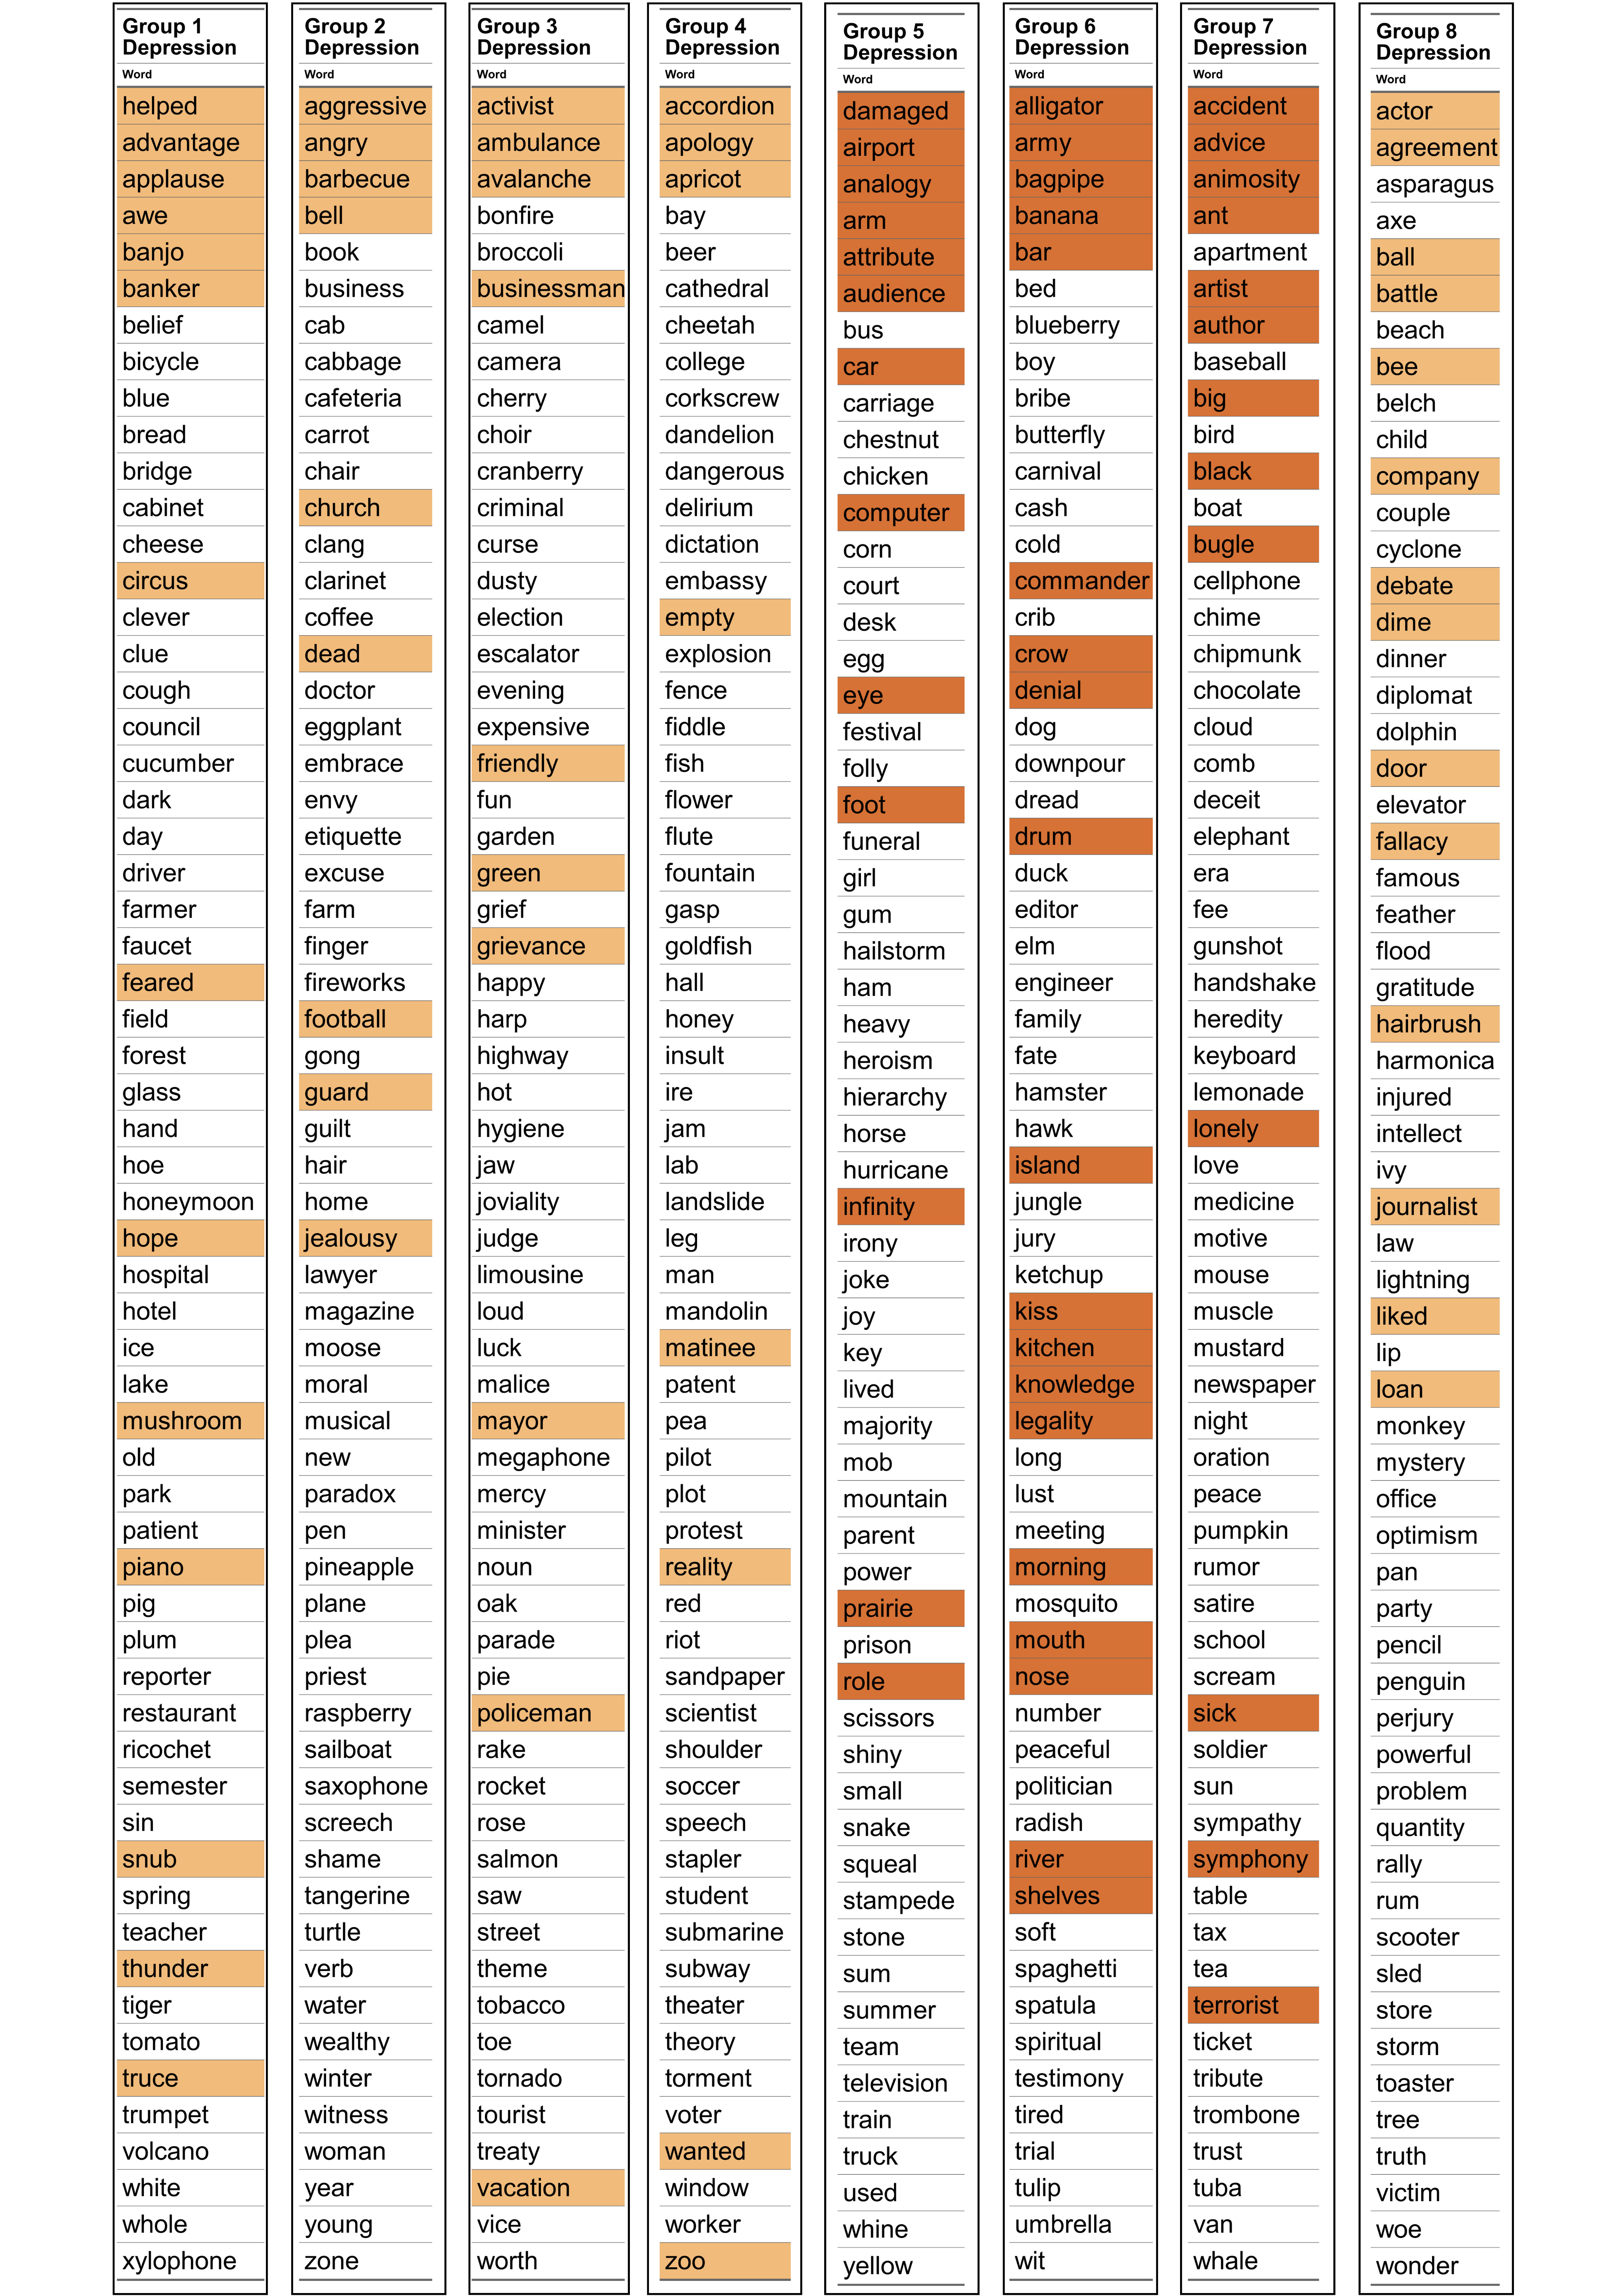
\includegraphics[width=0.90\textwidth]{figures/all_words_depr.png}
\caption*{Figure A1: Full list of words for each group. Words that were included in \textbf{depression}-classifiers that were significant in permutation test 1 on the train dataset are colored light brown. Words that were significant on train- \textit{and} holdout datasets are colored dark brown.}
\end{figure}

\begin{figure}
\centering
\vspace{-0.7cm}
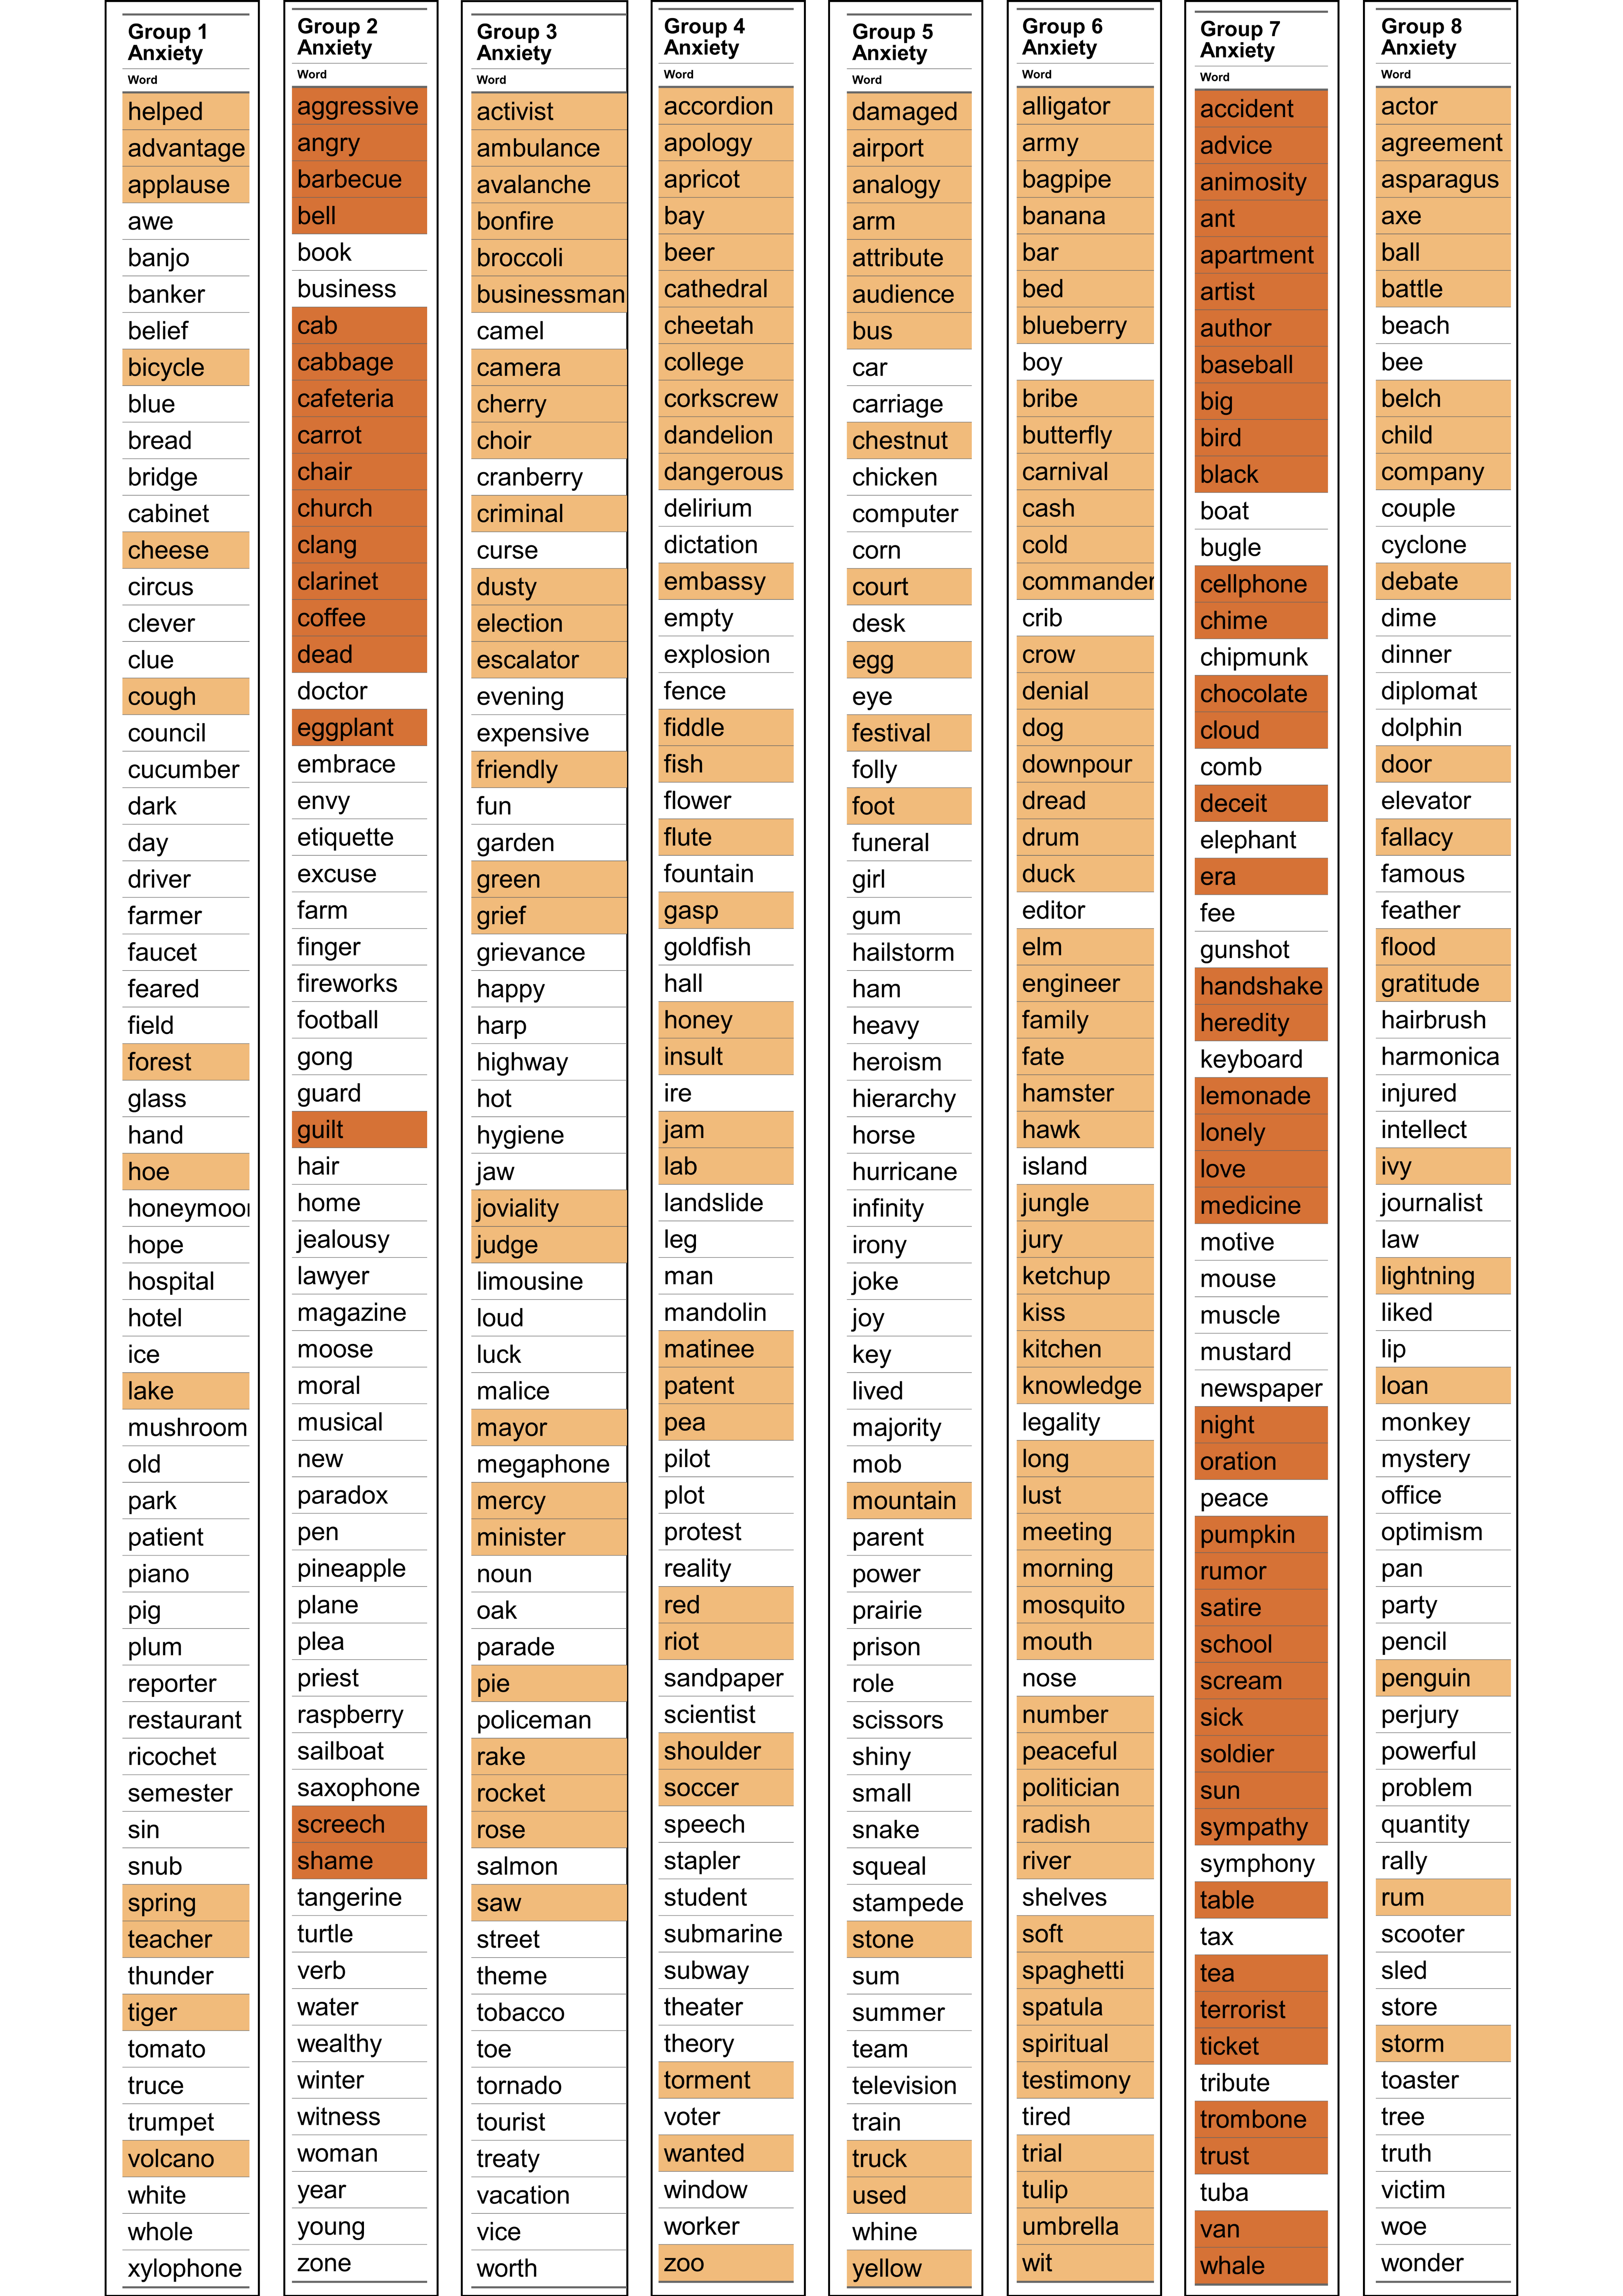
\includegraphics[width=1\textwidth]{figures/all_words_anx.png}
\caption*{Figure A2: Full list of words for each group. Words that were included in \textbf{anxiety}-classifiers that were significant in permutation test 1 on the train dataset are colored light brown. Words that were significant on train- \textit{and} holdout datasets are colored dark brown.}
\end{figure}

\newpage
\section{\\ Pairwise partial Kendall correlations of words in classifiers}

\begin{figure}[hbt!]
\centering
\vspace{-0.7cm}
\includesvg[width=1\textwidth]{figures/cm_d.svg}
\caption*{Figure B1: Pairwise partial Kendall correlations of words in \textbf{depression}-classifiers.}
\end{figure}

\begin{figure}
\centering
\vspace{-0.7cm}
\includesvg[width=1\textwidth]{figures/cm_a123.svg}
\caption*{Figure B2: Pairwise partial Kendall correlations of words in \textbf{anxiety}-classifiers for groups 1, 2, and 3.}
\end{figure}

\begin{figure}
\centering
\vspace{-0.7cm}
\includesvg[width=0.8\textwidth]{figures/cm_a45.svg}
\caption*{Figure B3: Pairwise partial Kendall correlations of words in \textbf{anxiety}-classifiers for groups 4 and 5.}
\end{figure}

\begin{figure}
\centering
\vspace{-0.7cm}
\includesvg[width=1\textwidth]{figures/cm_a6.svg}
\caption*{Figure B4: Pairwise partial Kendall correlations of words in the \textbf{anxiety}-classifier of group 6.}
\end{figure}

\begin{figure}
\centering
\vspace{-0.7cm}
\includesvg[width=1\textwidth]{figures/cm_a7.svg}
\caption*{Figure B5: Pairwise partial Kendall correlations of words in the \textbf{anxiety}-classifier of group 7.}
\end{figure}

\begin{figure}
\centering
\vspace{-0.7cm}
\includesvg[width=1\textwidth]{figures/cm_a8.svg}
\caption*{Figure B6: Pairwise partial Kendall correlations of words in the \textbf{anxiety}-classifier of group 8.}
\end{figure}


\newpage
\section{\\ Variance inflation factor scores of words in classifiers}

\begin{figure}[hbt!]
\centering
\vspace{-0.5cm}
\includesvg[width=1\textwidth]{figures/vif_d.svg}
\caption*{Figure C1: Variance inflation factor scores of words in \textbf{depression}-classifiers.}
\end{figure}

\begin{figure}
\centering
\vspace{-0.7cm}
\includesvg[width=1\textwidth]{figures/vif_a.svg}
\caption*{Figure C2: Variance inflation factor scores of words in \textbf{anxiety}-classifiers.}
\end{figure}




\end{document}